\documentclass[12pt, a4paper]{article}
\usepackage[utf8]{inputenc}

% indent first paragraph form new pages
\usepackage{indentfirst}

% margins
\usepackage[a4paper, left=3cm, right=2cm, top=2cm, bottom=2cm]{geometry}

% line space between lines
\renewcommand{\baselinestretch}{1.5}

% indent first sentence
\setlength{\parindent}{4em}

% indent between paragraphs
\setlength{\parskip}{0.7em}

% for figures
\usepackage{float}
\usepackage{graphicx}
\usepackage{caption, threeparttable}
\captionsetup{labelfont = sc, textfont = it, width=.8\linewidth}

% math helpers
\usepackage{amsmath}

% build images
\usepackage{tikz}
\usetikzlibrary{shapes,snakes, arrows.meta, fit, positioning}

% algorithm
\usepackage[linesnumbered,ruled]{algorithm2e}

\usepackage{listings}
\lstset{
  basicstyle=\ttfamily,
  columns=fullflexible,
  frame=single,
  breaklines=true,
  postbreak=\mbox{\textcolor{red}{$\hookrightarrow$}\space},
}

\newtheorem{obs}{Obs.}

\begin{document}
    % \large
    
    \begin{titlepage}
    \begin{center}
        
        UNIVERSITY OF PITESTI\\
        FACULTY OF SCIENCES,\\
        PHYSICAL EDUCATION AND INFORMATICS\\
        MASTER PROGRAM "ADVANCED TECHNIQUES FOR INFORMATION\\
        PROCESSING"
    
        \vskip 6cm
        
        {\LARGE\bf MASTER THESIS}
        
        \vskip 4.5cm
        
        \textbf{
            \begin{tabular}{ccc}
                Supervisor: &  \\
                Lect.univ.dr. Doru CONSTANTIN\\
                & Student's name: \\
                & Dragoș Ionuț RĂDUCANU \\
            \end{tabular}
        }
        
        \vskip 6cm
        
        \Large{-- 2018 --}
    \end{center}
\end{titlepage}

    \begin{titlepage}
    \begin{center}
        $ $
        \vskip 7cm
        
        {\LARGE\bf\sc 
            Data Processing by using Neural Techniques 
        }
    
    \end{center}
\end{titlepage}
    
    \newpage
    \tableofcontents
    
    \newpage
    \section*{Introduction}
\addcontentsline{toc}{section}{Introduction}


The human brain has been compared to an information processing system since ancient times. Since 1943, when Warren McCulloch and Walter Pitts presented the first model of artificial neurons. New and more sophisticated proposals have been made from one decade to the next. The mathematical analysis solved some of the mysteries represented by the new models, but left many open questions for future investigations.

The study of neurons, and their interconnections is one of the most dynamic and important fields of research in modern biology. The human brain can be considered faster and more powerful than the most powerful super computer ever built by humans. He has the ability to organize his neural activity in such a way as to perform complex activities: form recognition, perception, motor control, etc. The brain succeeds in about 100-200 ms. to solve a complex problem like that of recognizing a person, while a computing system requires much more time for simpler tasks. The question "How does the human brain work? " Is far from being known.

Artificial neural networks are an attempt to model the capacity of the nervous system to process information. Taking into account the essential properties of biological neural networks in terms of information, abstract models of artificial neural networks can be designed, which can then be simulated and analyzed.

Perceptron with a single layer is the simplest neural network. This elementary and simple network has the ability to learn to recognize simple forms. The simple perceptron teaches with the help of a supervised learning law how to learn. The simple Perceptron architecture consists of the input layer and the exit layer. It haven't hidden layers.

From the Perceptron model, other neural networks, including the BackPropagation network, have been developed. BackPropagation networks are direct-acting neural networks. That contain input nodes, ouput nodes and one or more layers of nodes between these two. These additional layers represent the hidden levels of multilayer perceptrons.

This paper aims to put neural networks into practice for classifying text data.
 
In Chapter 1 there are some general notions about "neurons" and neural networks. Also are some of the areas covered by these neural networks and how their working.
 
in chapter 2 are presented two ways of learning neural networks (supervised learning and unsupervised learning). Here are some ways to optimize neural networks. These are perfect for shortening your learning time as well as increasing your success rate. It will also show how recurring neural networks work to classify text data.
 
In Chapter 3 will be implemented a model for classifying text data. Python will be used for this. To ease the construction of the neural model, the Tensor Flow framework will be used. Also, the performance of the algorithm will be highlighted by altering different neural optimization. The model will also be tested with pre-trained Glove data. Glove is an unsupervised neural network.
    
    \newpage
    \section{Generalities}

\subsection{Biologic neuron}

The human brain is a complex system that coordinates the behavior of the body. He could not be matched by any digital structure.

The functional unit of the creature is the neuron. In the human brain there are about $ 10 ^ {11} $ neurons. They transmit and receive electro-chemical signals.

A neuron is composed of: \cite{toulouse}:
\begin{itemize}
    \item A cell body (soma).
    \item Dendrite, which fulfills the input function, capture information.
    \item Axon, an extension of the neuron body, with output function.
\end{itemize}

The dendritic tree collects the input signals from other neurons; soma converts the input signals into output signals, and the axon transmits the output signals to other neurons. Neurons are interconnected with synapses.

Neurons communicate with each other through electrical signals. These are propagated along the axon until they encounter the synaptic bond. Dendrites of the biological neuron receive electrical signals from the axons of other neurons.

Neurotransmitter molecules reach the post-synaptic neuron membrane, where the intake of these molecules induce post-synaptic action potential (PSP) \cite{calculNeuronal}.

PSPs generated at various points of the dendritic tree diffuse through attenuation to the soma, where they are integrated. If the total amount of PSPs embedded within a short time span exceeds a certain threshold of about a few tens of minivolts, called activation level, the neuron will become active, generating a potential for action along the axon.

The contribution of an input signal to PSP characterizes the size called synaptic strength or synaptic efficiency. Such an input signal has a value of about 1 minivolt, which may be an excitatory signal or an inhibitory signal, depending on the positive or negative influence it has on making a neuron to become active. We must point out that the PSP is not unique determined by the input signal. Different noise sources, in relation to the chemical neurotransmitter quantity fluctuations released on the synaptic connection, involve a probabilistic input-output relationship.

The time interval between the moment of a signal transmission to the pre-synaptic neuron soma and the time of emission of a signal induced by the postsynaptic neuron is approximately 1-2 ms. It follows that a neuron can have a maximum emission of about 500-1000 signals per second, which is reduced by about 3-5 times in a neural network.

From these dynamics considerations of neuronal activity, one can notice that biological neuron is a slow biological device compared to man-made electronic devices - they can be even hundreds of thousands of times faster than a biological neuron. However, any computer-based computing system has lower brain performance than neurons. The obvious conclusion is that the computing power of the human brain is not due to the processing speed of constitutive neurons but to the wide interconnection of slow biological devices - neurons, which perform simple operations: integration of incoming signals along the dendritic tree and emission of a signal along the axon, if the integrated input signal exceeds the activation level \cite{calculNeuronal}.

\begin{figure}[H]
  \centering
  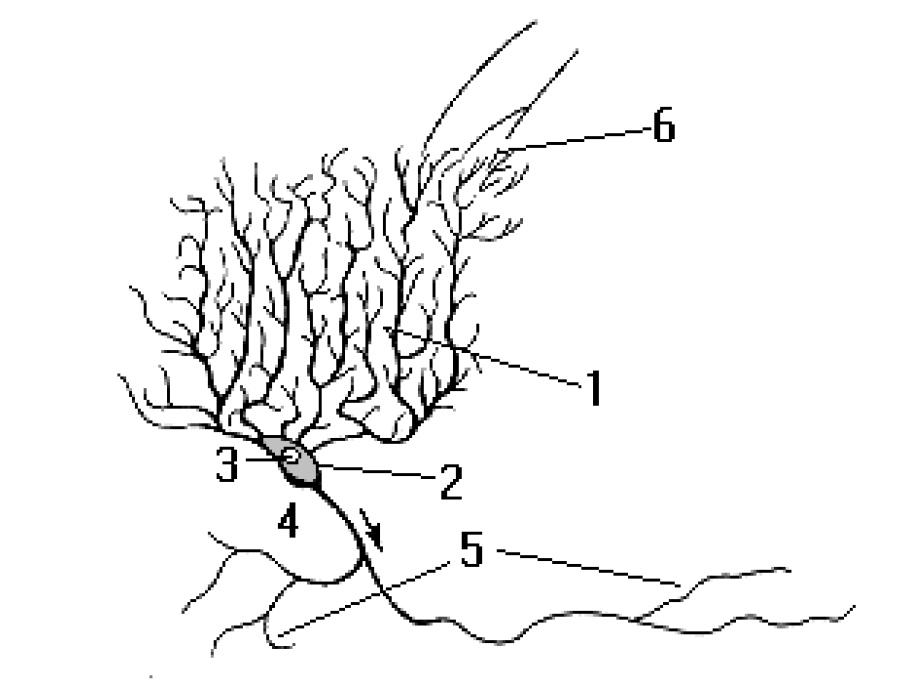
\includegraphics[width=3.5in]{images/neuronulBiologic.png}
  \caption {
      Schematic representation of the biological neuron.\\ 
      1 - The dendritic tree;\\ 
      2 - Soma (cell body);\\ 
      3 - The core of the neuronal cell;\\ 
      4 - The axon;\\ 
      5 - The axon tree;\\ 
      6 - Synaptic connections.
  }
\end{figure}

Changing synaptic strength is the result of a "learning" process \cite{calculNeuronal}. Link synaptic and signal processing by the neuron form the mechanism of based on the memory capacity of the brain.
\subsection{Artificial neuron}

As model for the artificial neuron was biological neuron.

An artificial neuron has several input paths that represent the dendritic tree of the biological neuron. For each input path $ i $ in the $ j $ neuron corresponds to a numeric value $ x_i $. This numerical value is the correspondent of the electrical signal from the biological neuron model. Each value $ x_i $ corresponds to the real numerical value $ w_ {ji} $ which is the equivalent of the synaptic force in the biological model of the neuron.

The product $ x_i \ cdot w_ {ji} $ represents the signal $ i $ entering the artificial neuron $ j $.

The sum of $ \ sum_ {i} ^ {} x_i \ cdot w_ {ji} $ represents the argument of the activation function that determines the axonic output value $ y_j $ from the neuron \cite{calculNeuronal}. The most commonly used activation functions are:

\begin{itemize}
  \item linear function: $$f \colon \mathcal{R} \to \mathcal{R}, f(x)=x$$
  \item step function (Heaviside): $$f \colon \mathcal{R} \to \{0,1\}, 
    f(x)= \begin{cases} 
            1, & x \geq 0 \\ 
            0, & x < 0 
          \end{cases}$$
  \item sigmoidal function: $$f \colon \mathcal{R} \to (0,1), f(x)=\frac{1}{1+e^{-x}}$$
  \item signum function: $$f \colon \mathcal{R} \to \{-1,1\}, f(x)=sgn(x)=
          \begin{cases} 
            1, & x \geq 0 \\ 
            -1, & x < 0 
          \end{cases}$$
  \item hyperbolic tangent function: $$f \colon \mathcal{R} \to (-1,1), f(x)=tanh(x)=\frac{e^x-e^{-x}}{e^x+e^{-x}} $$
\end{itemize}

Depending on the type of problem we want to solve, you can choose an activation function. These are examples of activation functions that are most commonly used in practical applications. The activation function depends on the chosen neural network model and the type of problem we want to solve, and its choice is not constrained by any condition except eventual analogy with the biological model.

The value obtained by applying the activation function is propagated on the output paths, equivalent to the axonal shaft of the biological model \cite{calculNeuronal}.

In \figurename{ \ref{fig:artificialNeuron}} we have the schematic representation of the artificial neuron.

In conclusion, the artificial neuron performs the following operations:

\begin{itemize}
    \item Input: $$ I_j = \sum_{i=0}^{n} x_i \cdot w_{ji} $$
    \item Activation: $$ y_j = f(I_j) = f(\sum_{i=0}^{n} x_i \cdot w_{ji}) $$
\end{itemize}


\begin{figure}[H]
    \centering
    \resizebox{10cm}{!}{\tikzset{%
  neuron/.style={
    circle,
    draw,
    minimum size=1cm
  },
  neuron missing/.style={
    draw=none, 
    scale=4,
    execute at begin node=\color{black}$\vdots$
  },
  neuron activation/.style={
    circle split,
    draw,
    rotate=90,
    minimum size=4cm
  }
}

\begin{tikzpicture}[x=3cm, y=2cm]

    \foreach \m [count=\y] in {1,2,missing,3,missing,4}
      \node [neuron/.try, neuron \m /.try] (input-\m) at (0,1.5-\y) {};
    
    \node [neuron activation/.try ] (output-1) at (2,-2) {
        \rotatebox{-90}{Sum \ $I_j$} 
        \nodepart{lower} 
        \rotatebox{-90}{Activation \ $f(I_j)$}
    };
      
     
    \foreach \l [count=\i] in {0,1,i,n}
      \draw [<-] (input-\i) -- ++(-1,0)
        node [above, midway] {$x_\l$};
    
    
    \foreach \k [count=\i] in {0,1,i,n}
        \draw [->] (input-\i) -- (output-1)
            node [above, midway] {$w_{j\k}$};
            
            
    \draw [->] (output-1) -- (3.5,-2)
      node [above, midway] {$y_j$};

\end{tikzpicture}}
    \caption{Semantic representation of semantic neuron}
    \label{fig:artificialNeuron}
\end{figure}

\begin{obs}
\label{obs:bias}
    The term $ x_0 $ is called bias, with a constant value of $ x_0 $ = +1 or $ x_0 $ = -1. The role of the bias term is to allow implicit or explicit inclusion of activation level $ \theta_i $, which represents the threshold of activation of the artificial neuron \cite{calculNeuronal}.
\end{obs}

For example, assuming we have the signum activation function,
$$f(x)=
  \begin{cases} 
    1, & x \geq 0 \\ 
    -1, & x < 0 
  \end{cases}$$
then we can have one of the following situations:\\
\begin{enumerate}
    \item Activation level $\theta_j$ explicit:
        \begin{itemize}
            \item Integration (Sum): $$ I_j = \sum_{i=0}^{n} x_i \cdot w_{ji} \geq \theta_j $$
            \item Activation (Transfer): $$ y_j = f(I_j) = f(\sum_{i=0}^{n} x_i \cdot w_{ji}) $$
        \end{itemize}
    \item Activation level $\theta_j$ implicit: we note $w_{j0} = \theta_j, x_0 = -1$
        \begin{itemize}
            \item Integration (Sum): $$ I_j = \sum_{i=0}^{n} x_i \cdot w_{ji} \geq 0 $$
            \item Activation (Transfer): $$ y_j = f(I_j) = f(\sum_{i=0}^{n} x_i \cdot w_{ji}) $$
        \end{itemize}
\end{enumerate}


This mathematical model of the artificial neuron, proposed for the first time by McCullogh and Pitts \cite {autoriFundamentali}, though very simple, are a very powerful computing unit.

McCullogh and Pitts have demonstrated that a set of interconnected artificial neurons is capable in principle of making any calculation, subject to the appropriate choice of strengths synaptic $ w_{ji} $. This means that an ensemble of artificial neurons interconnected into a an assembly called a neural network, can perform any calculation that one can perform classical computing system, though not always as fast or convenient.
\subsection{Areas of use of neural networks}

\subsubsection{Processing of natural languages}

Understanding natural languages allows people to interact with computers without special knowledge.

D. Rumelhart and J. McClelland \cite{Rumelhart} introduced neural networks in the field of natural language processing. By processing a natural language we will understand the study of how to construct the rules of a language.

D. Rumelhart and J. McClelland studied a language learning model with the help of a neural network able to teach English past Past Tense. By learning the neural network, it has progressed from a beginner's stage that brings bring-broughted mistakes to a phase of specialist in which she was able to determine the time for irregular verbs. The ability of the neural network to generalize on the basis of incomplete data and self-organization has allowed the neural network to generate correct responses when a new or unknown verb was presented.

\subsubsection{Compression of multidimensional data}

G. W. Cottrell, D. Zipser and P. Munro \cite{Cottrell} used neural networks to efficiently compress information corresponding to graphical images. The graphical images occupy, according to the resolution of the representation and the number of colors used, a very large storage space, reaching the order of the mega-bytes.

Image compression is a practical necessity because the storage space is very expensive and at the same time the transfer time of an image is obviously influenced by the amount of memory space required for that image.

The neural computer system designed by Cottrell, Munro, and Zipser is based on a three-layer neural network capable of compressing an image, and of course able to decompress it without distortion. It is important to note the unsupervised learning law used to learn the neural network, which allowed it to self-configure without the intervention of specialists. With this neural network, data compression has been accomplished eight times, with an impeccable decompression of the original image.


\subsubsection{Character Recognition}

An important area of use of neural networks is the field of visual interpretation and symbol classification \cite{Bishop}.

\paragraph{Handwriting recognition.} Researchers at Nestor Inc. in the US, have developed a neural computer system that has as a data entry device a digitizing tablet, which can be written using a Light-Pen. The neural network was trained with different handwriting, being able to interpret some handwriting with a high degree of acuity.

There are a large number of optical character recognition systems called OCR (Optical Character Recognition) \cite{oecd}. What differentiates neural networks from traditional OCR systems is flexibility. After learning, the neural network is able to recognize a great variety of writings and make pertinent assumptions about confusing characters.

Nestor's researchers built a neural network for Japanese writing (Kanji). It has been possible to eliminate the difficulty of quantifying the specific elements of a language by using neural networks in this area.

\paragraph{Image processing.} K. Fukushima \cite{Fukushima1,Fukushima2} has developed a neural imaging system for image recognition with practical applicability in the field of character recognition. The built-in neural network is based on an advanced form recognition system called Neocognitron.

Neocognitron is actually a multi-layer neural network. That simulates the way the human cortex is processed. The successively hidden neurons of Neocognitron are designed to extract defining features of the image without being influenced by orientation or distortion. At the input layer level, shapes are uniquely determined, with the information being propagated to the output layer, only certain neurons corresponding to some defining features of the image being activated.


    
    \newpage
    \section{Machine learning}

Machine learning (ML) is a type of artificial intelligence (AI) that allows software applications to become more accurate in predicting outcomes without being explicitly programmed. The basic premise of machine learning is to build algorithms, very efficient, that can receive input data and use statistical analysis to predict an output value within an acceptable range.

Machine learning algorithms are often categorized as being supervised or unsupervised. Supervised algorithms require humans to provide both input and desired output, in addition to furnishing feedback about the accuracy of predictions during training. Once training is complete, the algorithm will apply what was learned to new data. Unsupervised algorithms don't need to be trained with desired outcome data. Instead, they use an iterative approach called deep learning to review data and arrive at conclusions. Unsupervised learning algorithms are used for more complex processing tasks than supervised learning systems.

\subsection{Supervised learning}

One of the main types of automatic learning is supervised learning. This type of learning is akin to human learning based on the acquisition of new knowledge and skills through the experiences of the past. That means, the computer learns from data it has previously collected.

Changing the synaptic forces is based on the comparison between the output vector $ y ^ t = (y ^ t_1, y ^ t_2, ..., y ^ t_m), t = 1, ..., P $ obtained at the output layer and the target vector $ z ^ t = (z ^ t_1, z ^ t_2, ..., z ^ t_m), t = 1, ..., P $, representing the desired result to be obtained at the output layer, at the input layer the input vector $ x ^ t = (x ^ t_0, x ^ t_1, x ^ t_2, ..., x ^ t_n), t = 1, ..., P $ of the training.

The target vector $ z ^ t $ is provided by a teacher (coach-supervisor), hence the supervised learning name. Supervised learning involves the presentation by a coach of pairs of data form $ (x ^ t, z ^ t), t = 1, ..., P $ forming a set of data, called training set: $$ S = \{(x ^ t, z ^ t) | t = 1, ..., P \} $$

The difference between the obtained y response and the desired z response is the error and is used to modify the synaptic forces, based on a specific algorithm called \cite{calculNeuronal}.

We can represent supervised learning with the following diagram \cite{Baum}:

\begin{figure}[H]
  \centering
  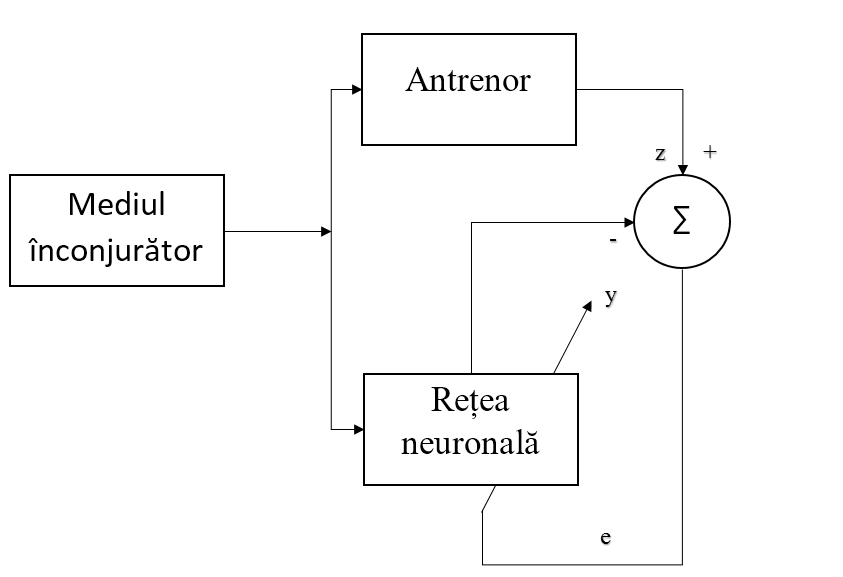
\includegraphics[width=3.5in]{images/diagramaInvSupervizate.png}
  \caption {Diagram of supervised learning.}
\end{figure}

It is seen from this diagram the equivalence of the supervised learning paradigm with the learning algorithm based on minimizing the error function \cite{Haykin}.
\subsection{Unsupervised learning}

Unsupervised learning involves learning without a coach \cite{Girolami}. The neural network must be able to "discover" patterns, features, correlations or categories in the input data set themselves and encode them in the form of output data \cite{Sanger1, Sanger2}. Neural network connections and neurons must represent a degree of self-organization.

Unsupervised learning can only be used when there is redundancy in the input data set. Without redundancy, it is impossible to discover any pattern or trait in the set of input data. From this point of view, redundancy ensures knowledge \cite{Barlow}.

The diagram below is the paradigm of unsupervised learning:

\begin{figure}[H]
  \centering
  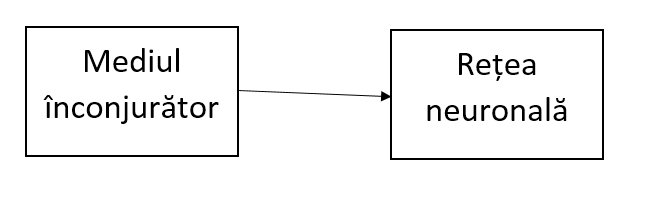
\includegraphics[width=3in]{images/diagramaInvNesupervizate.png}
  \caption {Unsupervised Learning Diagram.}
\end{figure}

In unsupervised learning, we have information about a measure of the quality of representation that the neural network needs to reach through the learning process \cite{Diamantaras}. Its parameters will be optimized for this measure. If the learning process is over, the neural network will be able to form internal representations that encode the input data features and automatically create new classes \cite{Diamantaras}.

We can use a competitive learning algorithm or a Hebbian learning algorithm for a neural network to be able to perform unsupervised learning.
\subsection{Learning optimizer}

Optimization refers to the task of minimizing/maximizing an objective function $f(x)$ parameterized by $x$. In machine/deep learning terminology, it’s the task of minimizing the cost/loss function $J(w)$ parameterized by the model’s parameters $w \in R^d$. Optimization algorithms (in case of minimization) have one of the following goals:

\begin{itemize}
    \item Find the lowest possible value of the objective function within its neighborhood. That’s usually the case if the objective function is not convex as the case in most deep learning problems.
    \item Find the global minimum of the objective function. This is feasible if the objective function is convex, i.e. any local minimum is a global minimum.
\end{itemize}

There are three kinds of optimization algorithms:

\begin{itemize}
    \item Optimization algorithm that is iterative in nature and converges to acceptable solution regardless of the parameters initialization such as gradient descent applied to logistic regression.
    \item Optimization algorithm that is iterative in nature and applied to a set of problems that have non-convex cost functions such as neural networks. Therefore, parameters’ initialization plays a critical role in speeding up convergence and achieving lower error rates.
    \item Optimization algorithm that is not iterative and simply solves for one point.
\end{itemize}

\subsubsection{Adam optimizer}

The method computes individual adaptive learning rates for different parameters from estimates of first and second moments of the gradients; the name Adam is derived from adaptive moment estimation. This is used to perform optimization and is one of the best optimizer at present. The author claims that it inherits from RMSProp and AdaGrad (Well it inherits from them).\\

Features:
\begin{itemize}
    \item The step-size is approximately bounded by the step-size hyper-parameter.
    \item It doesn't require stationary objective. That means the f(x) we talked about might change with time and still the algorithm will converge.
    \item Parameters update are invariant to re-scaling of gradient. It means that if we have some objective function f(x) and we change it to $k*f(x)$ (where k is some constant). There will be no effect on performance.
    \item Naturally performs step size annealing. Well remember the classical SGD, we used to decrease step size after some epochs, nothing as such is needed here.
\end{itemize}

The method is straightforward to implement, is computationally efficient, has little memory requirements, is invariant to diagonal rescaling of the gradients, and is well suited for problems that are large in terms of data and/or parameters \cite{Diederik}. 

\begin{algorithm}
    \SetKwInOut{Input}{Input}
    \SetKwInOut{Output}{Output}

    \Input{$\alpha$: Stepsize}
    \Input{$\beta_1, \beta_2 \in [0, 1)$: Exponential decay rates for the moment estimates}
    \Input{$f(\theta)$: Stochastic objective function with parameters $\theta$}
    \Input{$\theta_0$: nitial parameter vector}
    
    $m_0 \leftarrow 0$ (Initialize $1^{st}$ moment vector)\;
    $v_0 \leftarrow 0$ (Initialize $2^{nd}$ moment vector)\;
    $t \leftarrow 0$ (Initialize timestep)\;
    
    \While {$\theta_t$ not converged} {
        $t \leftarrow t + 1$ \;
        $g_t \leftarrow \bigtriangledown_0 f_1 (\theta_{t-1})$ (Get gradients w.r.t. stochastic objective at timestept)\;
        $m_t \leftarrow \beta_1 \cdot m_{t-1} + (1 - \beta_1) \cdot g_t$ (Update biased first moment estimate)\;
        $v_t \leftarrow \beta_2 \cdot v_{t-1} + (1-\beta_2) \cdot g_t^2$ (Update biased second raw moment estimate)\;
        $\widehat{m}_t \leftarrow m_t/(1 - \beta_1^t)$ (Compute bias-corrected first moment estimate)\;
        $\widehat{v}_t \leftarrow v_t/(1 - \beta_2^t)$ (Compute bias-corrected second raw moment estimate)\;
        $\theta_t \leftarrow \theta_{t-1} - \alpha \cdot \widehat{m}_t / (\sqrt{\widehat{v}_t} + e)$ (Update parameters)\;
    }
    
    \Return $\theta_t$ (Resulting parameters)

    \label{alg:adamOptimizer}
    \caption{Adam, proposed algorithm for stochastic optimization.}
\end{algorithm}

Let $f(\theta)$ be  a  noisy  objective  function:  a  stochastic  scalar  function  that  is  differentiable  w.r.t. parameters $\theta$. We  are  interested in minimizing the expected value of this function, $E[f(\theta)]$ w.r.t. its parameters $\theta$. With $f_1(θ),...,f_T(θ)$ we  denote  the  realisations  of  the  stochastic  function  at  subsequent  timesteps 1,...,T. The stochasticity might come from the evaluation at random subsamples (minibatches) of datapoints, or arise from inherent function noise. With $g_t= \bigtriangledown_0 f_1 (\theta_{t-1})$ we denote the gradient, i.e. the vector of partial derivatives of $f_t.w.r.t \theta$ evaluated at timestep $t$. 

The algorithm updates exponential moving averages of the gradient $(m_t)$ and the squared gradient $(v_t)$ where the hyper-parameters $β_1,β_2 \in [0,1)$ control the exponential decay rates of these moving averages. The moving averages themselves are estimates of the $2^{nd}$ raw moment (the uncentered variance) and the $1^{st}$ moment (the mean) of the gradient.   However,  these moving averages are initialized as (vectors of) 0’s, leading to moment estimates that are biased towards zero, especially during the initial timesteps, and especially when the decay rates are small (i.e. the $\beta$s are close to 1).The good news is that this initialization bias can be easily counteracted, resulting in bias-corrected estimate $\widehat{m}_t$ and $\widehat{v}_t$.

Note that the efficiency of \ref{alg:adamOptimizer} can, at the expense of clarity, be improved upon by changing the order of computation, e.g.  by replacing the last three lines in the loop with the following lines \cite{Diederik}: $$\alpha_t = \alpha \cdot \sqrt{1 - \beta_2^t}/(1 - \beta_1^t)$$ and $$\theta_y \leftarrow \theta_{t-1} - \alpha_t \cdot m_t/(\sqrt{v_t} + \widehat{e})$$


\subsubsection{AdaGrad optimizer}

AdaGrad or adaptive gradient allows the learning rate to adapt based on parameters. It performs larger updates for infrequent parameters and smaller updates for frequent one. Because of this it is well suited for sparse data (NLP or image recognition). Another advantage is that it basically eliminates the need to tune the learning rate. Each parameter has its own learning rate and due to the peculiarities of the algorithm the learning rate is monotonically decreasing. This causes the biggest problem: at some point of time the learning rate is so small that the system stops learning.

\subsubsection{Gradient descendent optimizer}

Gradient Descent is the most common optimization algorithm in machine learning and deep learning. It is a first-order optimization algorithm. This means it only takes into account the first derivative when performing the updates on the parameters. On each iteration, we update the parameters in the opposite direction of the gradient of the objective function J(w) w.r.t the parameters where the gradient gives the direction of the steepest ascent. The size of the step we take on each iteration to reach the local minimum is determined by the learning rate $\alpha$. Therefore, we follow the direction of the slope downhill until we reach a local minimum.

\subsubsection{RMSprop optimizer}

Gradients of very complex functions like neural networks have a tendency to either vanish or explode as the energy is propagated through the function. And the effect has a cumulative nature; the more complex the function is, the worse the problem becomes.

Rmsprop is a very clever way to deal with the problem. It uses a moving average of squared gradients to normalize the gradient itself. That has an effect of balancing the step size; decrease the step for large gradient to avoid exploding, and increase the step for small gradient to avoid vanishing.
\subsection{Recurrent neural network}

Humans don’t start their thinking from scratch every second. As you read this essay, you understand each word based on your understanding of previous words. You don’t throw everything away and start thinking from scratch again. Your thoughts have persistence.

Traditional neural networks can’t do this, and it seems like a major shortcoming. For example, imagine you want to classify what kind of event is happening at every point in a movie. It’s unclear how a traditional neural network could use its reasoning about previous events in the film to inform later ones.

Recurrent neural networks address this issue. They are networks with loops in them, allowing information to persist.

\begin{figure}[H]
    \centering
    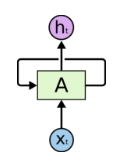
\includegraphics[width=2in]{images/rnn.png}
    \caption{Recurrent Neural Networks with loops.}
    \label{fig:rnnRoll}
\end{figure}

In the above diagram, a chunk of neural network, $A$, looks at some input $x_t$ and outputs a value $h_t$. A loop allows information to be passed from one step of the network to the next.

These loops make recurrent neural networks seem kind of mysterious. However, if you think a bit more, it turns out that they aren’t all that different than a normal neural network. A recurrent neural network can be thought of as multiple copies of the same network, each passing a message to a successor. Consider what happens if we unroll the loop:

\begin{figure}[H]
    \centering
    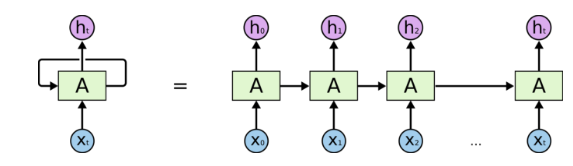
\includegraphics[width=6.5in]{images/rnnUnroll.png}
    \caption{Unrolled recurrent neural network.}
    \label{fig:rnnUnroll}
\end{figure}

This chain-like nature reveals that recurrent neural networks are intimately related to sequences and lists. For such data, they are the natural architecture of neural network.

And they certainly are used! In the last few years, there have been incredible success applying RNNs to a variety of problems: speech recognition, language modeling, translation, image captioning… The list goes on.

Over the years researchers have developed more sophisticated types of RNNs to deal with some of the shortcomings of the vanilla RNN model. I want this section to serve as a brief overview so that you are familiar with the taxonomy of models.

\subsubsection{Bidirectional RNNs}

Bidirectional recurrent neural networks(RNN) are really just putting two independent RNNs together. The input sequence is fed in normal time order for one network, and in reverse time order for another. The outputs of the two networks are usually concatenated at each time step, though there are other options, e.g. summation.

\begin{figure}[H]
    \centering
    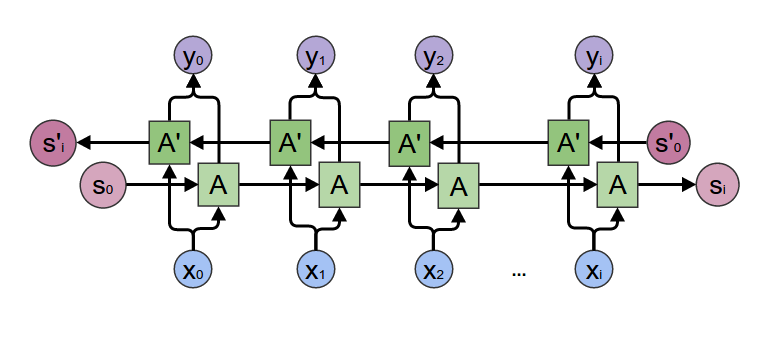
\includegraphics[width=6.5in]{images/bidirectionalRNN.png}
    \caption{General Structure of Bidirectional Recurrent Neural Networks.}
    \label{fig:bidirectionalRNN}
\end{figure}

This structure allows the networks to have both backward and forward information about the sequence at every time step.

They're often used when we’re trying to make predictions in a sequence. For example, in voice recognition, we might wish to predict a phenome for every time step in an audio segment, based on past context.

\subsubsection{Deep (Bidirectional) RNNs}

They're similar to Bidirectional RNNs, only that we now have multiple layers per time step. In practice this gives us a higher learning capacity (but we also need a lot of training data).

\subsubsection{LSTM networks}

One of the appeals of RNNs is the idea that they might be able to connect previous information to the present task. That work such as using previous video frames might inform the understanding of the present frame. If RNNs could do this, they’d be extremely useful. But can they? It depends.

Sometimes, to perform the present task, we only need to look at recent information. For example, consider a language model trying to predict the next word based on the previous ones. We don’t need any further context if we are trying to predict the last word in “the clouds are in the sky,”. – it’s pretty obvious the next word is going to be sky. In such cases, where the gap between the relevant information and the place that it’s needed is small, RNNs can learn to use the past information.


\begin{figure}[H]
    \centering
    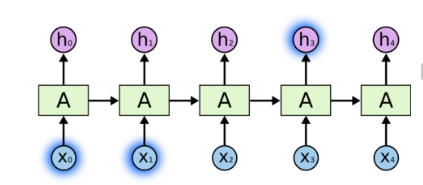
\includegraphics[width=4.5in]{images/rnnWhatWeNeed.png}
    \caption{Graphics representation for connecting informations}
\end{figure}


But there are also cases where we need more context. Consider trying to predict the last word in the text “I grew up in France… I speak fluent French.” Recent information suggests that the next word is probably the name of a language, but we need the context of France, from further back if we want to narrow down which language. It’s entirely possible for the gap between the relevant information and the point where it is needed to become very large.

Unfortunately, as that gap grows, RNNs become unable to learn to connect the information.

\begin{figure}[H]
    \centering
    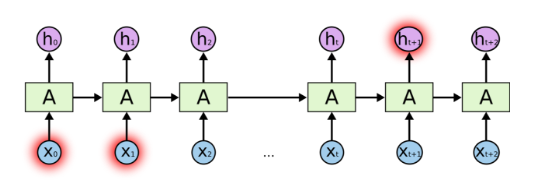
\includegraphics[width=6.5in]{images/rnnWhatWeNeedButCannot.png}
    \caption{Graphics representation for connecting informations, more data}
\end{figure}

In theory, RNNs are absolutely capable of handling such “long-term dependencies.” A human could carefully pick parameters for them to solve toy problems of this form. Sadly, in practice, RNNs don’t seem to be able to learn them. The problem was explored in depth by Hochreiter (1991) [German] and Bengio, et al. (1994), who found some pretty fundamental reasons why it might be difficult. \cite{lstm}

Thankfully, LSTMs don’t have this problem!

Long Short Term Memory networks – usually just called "LSTMs" – are a special kind of RNN, capable of learning long-term dependencies. They were introduced by Hochreiter \& Schmidhuber in 1997, and were refined and popularized by many people in following work. They work tremendously well on a large variety of problems, and are now widely used.

LSTMs are explicitly designed to avoid the long-term dependency problem. Remembering information for long periods of time is practically their default behavior, not something they struggle to learn!

All recurrent neural networks have the form of a chain of repeating modules of neural network. In standard RNNs, this repeating module will have a very simple structure, such as a single tanh layer.

\begin{figure}[H]
    \centering
    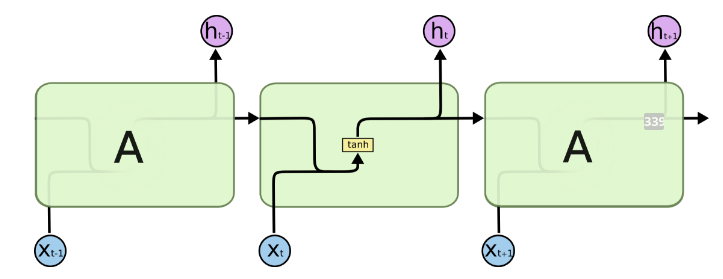
\includegraphics[width=6.5in]{images/rnnStandard.png}
    \caption{The repeating module in a standard RNN contains a single layer.}
\end{figure}

LSTMs also have this chain like structure, but the repeating module has a different structure. Instead of having a single neural network layer, there are four, interacting in a very special way.

\begin{figure}[H]
    \centering
    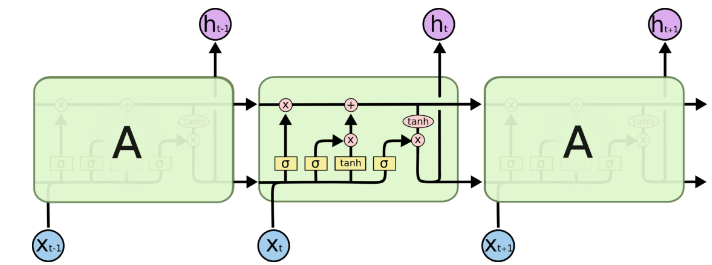
\includegraphics[width=6.5in]{images/lstm.png}
    \caption{The repeating module in an LSTM contains four interacting layers.}
\end{figure}

\subsection{Conditional random field}

Conditional Random Fields is a discriminative undirected probabilistic graphical model, a sort of Markov random field. The most often used for NLP version of CRF is linear chain CRF. CRF is a supervised learning method.

Linear chain CRF is good for different segmentation and sequence tagging tasks:

\begin{itemize}
    \item Keywords extraction
    \item (Named) Entity Recognition
    \item Sentiment Analysis
    \item Part-of-Speech Tagging
    \item Speech Recognition
\end{itemize}

The time complexity of the training process is large enough.
\begin{equation*} O(mNTQ2nS) \end{equation*}
, where:
\begin{itemize}
    \item m is the number of training iterations\
    \item N is the number of training data sequences
    \item T is the average length of training sequences
    \item Q is the number of class labels
    \item n is the number of CRF features
    \item S is the searching time of the optimization algorithm (for example, L-BFGS algorithm, which is considered good for this).
\end{itemize}

In practical implementation, the computational time is often larger due to many other operations like numerical scaling, smoothing etc. The time complexity of the inference process is much better in case of using Viterbi algorithm for inference:
\begin{equation*} О(T|S|^3) \end{equation*}
, where:

\begin{itemize}
    \item T is the number of training data sequences
    \item S is the number of class labels
\end{itemize}

The most similar method for CRF is MEMM (Maximum-entropy Markov Model). It is also discriminative probabilistic graphical model. However, MEMM has so called “label bias problem”. CRF has no such problem and this fact is the main difference between CRF and MEMM. It is not correct to compare CRF and HMM in direct way, because both CRF and HMM relate to different classes of algorithms – HMM is generative model and CRF is discriminative model.

The most evident disadvantage of CRF is high computational complexity of the training stage of the algorithm. This fact makes it more difficult to re-train the model when new training data samples become available. CRF does not work with unknown words, i.e. with words that were not present in training data sample.

Many researches show that CRF is better for NER task than MEMM and HMM. That is why Stanford NER is based on CRF. It is possible to reach high quality of labeling (e.g. for NER task) if you choose right features
CRF is flexible enough in terms of feature selection. In addition, it is not necessary for features to be conditionally independent.

\subsubsection{Keyword extraction}

As CRF is supervised machine learning algorithm, you need to have large enough training sample to train it. If you have such sample, and if you choose features wisely, theoretically you may obtain the quality around 0.6-0.7 (F1-measure)

Unfortunately, researches show us that in reality it is hardly unlikely to have a quality higher than 0.5 (F1-measure). For example, some Indian researchers used CRF to extract key words from medical texts and they had good features and large enough training sample, but they obtained quality not more than 0.4 (F1-measure). That’s sad.


\subsubsection{Named entity extraction}

CRF is significantly better in coping with NER task

For example, researchers from HSE and SPSU presented a paper, where they obtained quality of NER about 0.9 (F-measure) on a test set, having a training set not more than 70 000 examples. On real data they would hardly obtain such quality, while Stanford NER shows quality not more than 0.81 (F-measure) given it has perfectly selected training features and it was trained on larger corpora (CoNLL, MUC-6, MUC-7 and ACE)

Some Spanish and Russian researchers compared HMM and CRF in NER task for medical texts on JNLPBA corpus (18546 sentences with 109588 named entities). They obtained interesting results: HMM had higher recall (+4-7\% depending on the type of entity) while CRF had higher precision (+4-13\% depending on the type of entity). Average F-measure on cross-validation appeared to be about 0.65 for HMM and 0.69 for CRF. The authors supposed, that the quality of NER could have been 5-10\% higher if they used hybrid HMM+CRF algorithm.


\subsubsection{Time expressions extraction}

Time expressions are also entities, but very specific ones, so I decided to write about them in a separate section.

According to one master thesis, linear-chain CRF operated very well on extracting time expressions from Russian text. The author manually tagged 2000 sentences (which contained about 500 time expressions) then iteratively tuned parameters and features until he obtained 0.93 (F1-measure) in cross-validation.

Sounds cool, but in real process I think there would be no more than 0.7-0.75 (F1-measure). That is also very decent, though.

\subsubsection{Sentiment Analysis}

CRF copes with this task very well. Different research papers claim the results of using CRF for sentiment analysis for various languages are good enough – about 0.7 (F1-measure).

For instance, the researchers from HSE claimed that they achieved 0.74 (F1-measure) while performing Sentiment Analysis on real Twitter messages. They manually tagged 20 000 messages and achieved average 0.86 (F1-measure) on all three possible types of sentiment (positive, negative and neutral).

By the way, neutral class is important for a good sentiment analysis.


CRF is not very good for keywords extraction as soon as it cannot handle unknown words. Moreover, adding new data to the training dataset forcers us to re-train the whole CRF model – and it may be quite time-consuming due to the high complexity of the training phase of the algorithm.

CRF shows good performance when dealing with entity recognition (any types of entities, including named entities, time expressions, etc.). It can use both linguistic (characters, words) and non-linguistic information (upper/lower case, punctuation marks, spaces etc.). The achievable quality of entity recognition is about 0.7-0.85 (F1-measure), which is high.

There is an interesting idea to make a hybrid algorithm by combining HMM and CRF for entity recognition. Theoretically, such algorithm could increase overall quality of entity recognition by 5-10% and reach 0.85-0.9.
    
    \newpage
    \section{Implementation}

The paper aims to build a neural network for recognizing and classifying names from text data. For this, Python was used along with TensorFlow framework. Glove was introduced to boost performance. This unsupervised network created by standford, trains and creates links between words. Glove is very easy to use for training new data, such as rendering of words in other languages. In my case, there was enough standard data already trained by Standford. 

TensorBoard is another tool used to see the loss and how the graph (neural network) looks like.

\subsection{Why python?}

Python is an interpreted, object-oriented, high-level programming language with dynamic semantics. Its high-level built in data structures, combined with dynamic typing and dynamic binding, make it very attractive for Rapid Application Development, as well as for use as a scripting or glue language to connect existing components together. Python's simple, easy to learn syntax emphasizes readability and therefore reduces the cost of program maintenance. Python supports modules and packages, which encourages program modularity and code reuse. The Python interpreter and the extensive standard library are available in source or binary form without charge for all major platforms, and can be freely distributed.

Often, programmers fall in love with Python because of the increased productivity it provides. Since there is no compilation step, the edit-test-debug cycle is incredibly fast. Debugging Python programs is easy: a bug or bad input will never cause a segmentation fault. Instead, when the interpreter discovers an error, it raises an exception. When the program doesn't catch the exception, the interpreter prints a stack trace. A source level debugger allows inspection of local and global variables, evaluation of arbitrary expressions, setting breakpoints, stepping through the code a line at a time, and so on. The debugger is written in Python itself, testifying to Python's introspective power. On the other hand, often to add a few print statements to the source is the quickest way to debug a program: the fast edit-test-debug cycle makes this simple approach very effective.

Python language is one of the most flexible languages. It can be used for various purposes. Python has gained huge popularity base of this. Python does contain special libraries for machine learning namely scipy and numpy which great for linear algebra and getting to know kernel methods of machine learning. When want to work with machine learning algorithms python is great to use. It has easy syntax relatively. For beginners, this is the best language to use and to start with.

Whether a startup or an MNC, Python provides a huge list of benefits to all. The usage of Python is such that it cannot be limited to only one activity. Its growing popularity has allowed it to enter into some of the most popular and complex processes like Artificial Intelligence (AI), Machine Learning (ML), natural language processing, data science etc. The question is why Python is gaining such momentum in AI? And the answer lies below:

\begin{itemize}
    \item Less Code: AI involves algorithms - a LOT of them. Python provides ease of testing -  one of the best among competitors. Python helps in easy writing and execution of codes. Python can implement the same logic with as much as 1/5th code as compared to other OOPs languages. Thanks to its interpreted approach which enables check as you code methodology.
    \item Prebuilt Libraries: Python has a lot of libraries for every need of your AI project. Few names include Scipy for advanced computing, Numpy for scientific computation and Pybrain for machine learning. AIMA - is a library implemented in Python of algorithms from Russell and Norvig's 'Artificial Intelligence: A Modern Approach' is one of the best library available for Artificial Intelligence till today. Such a dedicated library saves developer’s time spent on coding base level items.
    \item Support: Python is a completely open source with a great community. There is a host of resources available which can get any developer up to speed in no time. There is a huge community of active coders willing to help programmers in every stage of developing cycle.
    \item Platform Agnostic: Python provides the flexibility to provide an API from an existing language which indeed provides extreme flexibility. It is also platform independent. With just a few changes in codes, you can get your app up and running in a new OS. This saves developers time in testing on different platforms and migrating code.
    \item Flexibility: Flexibility is one of the core advantages of Python. Python is suitable for every purpose with the option to choose between OOPs approach and scripting. It works as a perfect backend and it also suitable for linking different data structures together. A big plus for developers who are struggling between different algorithms is the option to check a majority of code in the IDE itself.
    \item Popularity: Python is winning the heart of millennials. It's ease of learning. Though AI Projects need a highly experienced programmer yet Python can smoothen the learning curve. It is practically more easy to look for Python developers than to hunt for LISP or Prolog programmers, particularly in some nations. Its extended libraries and active community with an ever developing and improving code have led it to be one of the hottest languages today.
\end{itemize}

Python is simple, elegant, consistent, and math-like.
\subsection{Tensor flow}

TensorFlow is an open source software library for high performance numerical computation. Its flexible architecture allows easy deployment of computation across a variety of platforms (CPUs, GPUs, TPUs), and from desktops to clusters of servers to mobile and edge devices. Originally developed by researchers and engineers from the Google Brain team within Google’s AI organization, it comes with strong support for machine learning and deep learning and the flexible numerical computation core is used across many other scientific domains.

Everything in TensorFlow is based on creating a computational graph. Think of a computational graph as a network of nodes, with each node known as an operation, running some function that can be as simple as addition or subtraction to as complex as some multi variate equation.

An Operation also referred to as op can return zero or more tensors which can be used later on in the graph. Heres a list of operations with their output for example.

Each operation can be handed a constant, array, matrix or n-dimensional matrix. Another word for an n-dimensional matrix is a tensor, a 2-dimensional tensor is equivalent to a m x m matrix.

\begin{figure}[H]
    \centering
    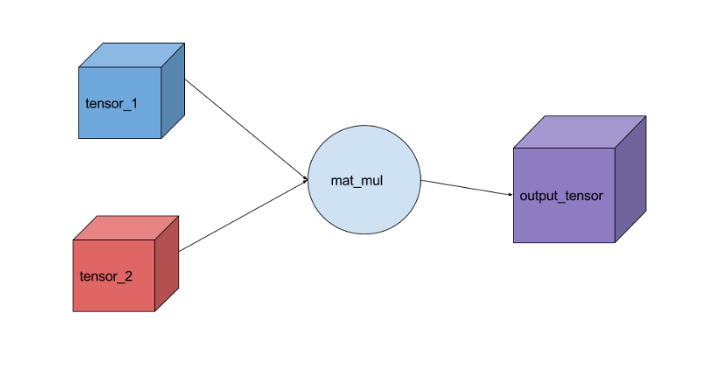
\includegraphics[width=6.5in]{images/tensor.png}
    \caption{Trivial tensor example.}
\end{figure}

The code above is creating two constant tensors and multiplying them together and outputting our result. This is a trivial example that demonstrates how you can create a graph and run the session. All inputs needed by the op are run automatically. They’re typically ran in parallel. This session run actually causes the execution of three operations in the graph, creating the two constants then the matrix multiplication.

\subsubsection{Graph}

The constants and operation was automagically added to the graph in TensorFlow. The graph default is instantiated when the library is imported. Creating a Graph object instead of using the default graph is useful when creating multiple models in one file that do not depend on each other.

\begin{lstlisting}[language=Python]
    new_graph = tf.Graph()
    with new_graph.as_default():
        new_g_const = tf.constant([1., 2., 3.])
\end{lstlisting}

any variables or operations used outside of the "with new\_graph.as\_default()" will be added to the default graph that is created when the library is loaded. You can even get a handle to the default graph with

\begin{lstlisting}[language=Python]
    default_g = tf.get_default_graph()
\end{lstlisting}

for most cases it’s best to stick with the default graph.

\subsubsection{Session}

This encapsulates the environment that operations and tensors are executed and evaluated. Sessions can have their own variables, queues and readers that are allocated. So it’s important to use the close() method when the session is over. There are 3 arguments for a Session, all of which are optional.

\begin{itemize}
    \item target: (Optional.) The execution engine to connect to. Defaults to using an in-process engine. 
    \item graph: (Optional.) The Graph to be launched. If no graph argument is specified when constructing the session, the default graph will be launched in the session. If you are using more than one graph (created with tf.Graph() in the same process, you will have to use different sessions for each graph, but each graph can be used in multiple sessions. In this case, it is often clearer to pass the graph to be launched explicitly to the session constructor.
    \item config: (Optional.) A ConfigProto protocol buffer with configuration options for the session.
\end{itemize}

\subsubsection{Placeholder}

As mentioned before, it all starts with placeholders. We need two placeholders in order to fit our model: X contains the network's inputs (the stock prices of all S\&P 500 constituents at time T = t) and Y the network's outputs (the index value of the S\&P 500 at time T = t + 1).

The shape of the placeholders correspond to [None, n\_stocks] with [None] meaning that the inputs are a 2-dimensional matrix and the outputs are a 1-dimensional vector. It is crucial to understand which input and output dimensions the neural net needs in order to design it properly.

\begin{lstlisting}[language=Python]
    # Placeholder
    X = tf.placeholder(dtype=tf.float32, shape=[None, n_stocks])
    Y = tf.placeholder(dtype=tf.float32, shape=[None])
\end{lstlisting}

The None argument indicates that at this point we do not yet know the number of observations that flow through the neural net graph in each batch, so we keep if flexible. We will later define the variable batch\_size that controls the number of observations per training batch.

\subsubsection{Variable}

Besides placeholders, variables are another cornerstone of the TensorFlow universe. While placeholders are used to store input and target data in the graph, variables are used as flexible containers within the graph that are allowed to change during graph execution. Weights and biases are represented as variables in order to adapt during training. Variables need to be initialized, prior to model training. We will get into that a litte later in more detail.

The model consists of four hidden layers. The first layer contains 1024 neurons, slightly more than double the size of the inputs. Subsequent hidden layers are always half the size of the previous layer, which means 512, 256 and finally 128 neurons. A reduction of the number of neurons for each subsequent layer compresses the information the network identifies in the previous layers. Of course, other network architectures and neuron configurations are possible but are out of scope for this introduction level article.

\begin{lstlisting}[language=Python]
    # Model architecture parameters
    n_stocks = 500
    n_neurons_1 = 1024
    n_neurons_2 = 512
    n_neurons_3 = 256
    n_neurons_4 = 128
    n_target = 1
    # Layer 1: Variables for hidden weights and biases
    W_hidden_1 = tf.Variable(
            weight_initializer(
                [n_stocks, n_neurons_1]))
    bias_hidden_1 = tf.Variable(
            bias_initializer(
                [n_neurons_1]))
    # Layer 2: Variables for hidden weights and biases
    W_hidden_2 = tf.Variable(
            weight_initializer(
                [n_neurons_1, n_neurons_2]))
    bias_hidden_2 = tf.Variable(
            bias_initializer(
                [n_neurons_2]))
    # Layer 3: Variables for hidden weights and biases
    W_hidden_3 = tf.Variable(
            weight_initializer(
                [n_neurons_2, n_neurons_3]))
    bias_hidden_3 = tf.Variable(
            bias_initializer(
                [n_neurons_3]))
    # Layer 4: Variables for hidden weights and biases
    W_hidden_4 = tf.Variable(
            weight_initializer(
                [n_neurons_3, n_neurons_4]))
    bias_hidden_4 = tf.Variable(
            bias_initializer(
                [n_neurons_4]))
    
    # Output layer: Variables for output weights and biases
    W_out = tf.Variable(
            weight_initializer(
                [n_neurons_4, n_target]))
    bias_out = tf.Variable(
            bias_initializer(
                [n_target]))
\end{lstlisting}

It is important to understand the required variable dimensions between input, hidden and output layers. As a rule of thumb in multilayer perceptrons (MLPs, the type of networks used here), the second dimension of the previous layer is the first dimension in the current layer for weight matrices. This might sound complicated but is essentially just each layer passing its output as input to the next layer. The biases dimension equals the second dimension of the current layer’s weight matrix, which corresponds the number of neurons in this layer.

\subsubsection{Scope}

Variables and tensors in TensorFlow have a name attribute that is used to identify them in the symbolic graph. If you don't specify a name when creating a variable or a tensor, TensorFlow automatically assigns a name for you:

\begin{lstlisting}[language=Python]
    a = tf.constant(1)
    print(a.name)  # prints "Const:0"
    
    b = tf.Variable(1)
    print(b.name)  # prints "Variable:0"
\end{lstlisting}

You can overwrite the default name by explicitly specifying it:

\begin{lstlisting}[language=Python]
    a = tf.constant(1, name="a")
    print(a.name)  # prints "a:0"
    
    b = tf.Variable(1, name="b")
    print(b.name)  # prints "b:0"
\end{lstlisting}

TensorFlow introduces two different context managers to alter the name of tensors and variables. The first is tf.name\_scope:

\begin{lstlisting}[language=Python]
    with tf.name_scope("scope"):
    a = tf.constant(1, name="a")
    print(a.name)  # prints "scope/a:0"
    
    b = tf.Variable(1, name="b")
    print(b.name)  # prints "scope/b:0"
    
    c = tf.get_variable(name="c", shape=[])
    print(c.name)  # prints "c:0"
\end{lstlisting}

Note that there are two ways to define new variables in TensorFlow, by creating a tf.Variable object or by calling tf.get\_variable. Calling tf.get\_variable with a new name results in creating a new variable, but if a variable with the same name exists it will raise a ValueError exception, telling us that re-declaring a variable is not allowed.

tf.name\_scope affects the name of tensors and variables created with tf.Variable, but doesn't impact the variables created with tf.get\_variable.

Unlike tf.name\_scope, tf.variable\_scope modifies the name of variables created with tf.get\_variable as well:

\begin{lstlisting}[language=Python]
    with tf.variable_scope("scope"):
        a = tf.constant(1, name="a")
        print(a.name)  # prints "scope/a:0"
        
        b = tf.Variable(1, name="b")
        print(b.name)  # prints "scope/b:0"
        
        c = tf.get_variable(name="c", shape=[])
        print(c.name)  # prints "scope/c:0"
  
    with tf.variable_scope("scope"):
        a1 = tf.get_variable(name="a", shape=[])
        a2 = tf.get_variable(name="a", shape=[])  # Disallowed
\end{lstlisting}

But what if we actually want to reuse a previously declared variable? Variable scopes also provide the functionality to do that:

\begin{lstlisting}[language=Python]
    with tf.variable_scope("scope"):
        a1 = tf.get_variable(name="a", shape=[])
    with tf.variable_scope("scope", reuse=True):
        a2 = tf.get_variable(name="a", shape=[])  # OK
\end{lstlisting}

\subsubsection{Loss}

Loss is the target function that the optimization algorithm will try to minimize.

In general, you want your loss function to be a measure of how bad your model is. But because the optimization algorithms require a few mathematical properties to work nicely, you can't pick the usual stuff like precision and recall (you want continuous functions that are differentiable in relation to the model parameters).

With classification tasks, softmax is a common choice. It's a smooth and well-behaved version of argmax, which is used to pick the class with highest network activation. With regression, the usual mean squared error serves fine.

\subsubsection{Logits}

Logit is a function. This will map probabilities [0, 1] to [-inf, +inf].

Softmax is a function that maps [-inf, +inf] to [0, 1] similar as Sigmoid. But Softmax also normalizes the sum of the values(output vector) to be 1.

Tensorflow "with logit": It means that you are applying a softmax function to logit numbers to normalize it. The input\_vector/logit is not normalized and can scale from [-inf, inf].

For multiclass classification problems is used this normalization. And sigmoid normalization is used for multilabel classification problems i.e. 
\begin{lstlisting}[language=Python]
    tf.nn.sigmoid_cross_entropy_with_logits
\end{lstlisting}

\subsubsection{Feed}

There are three main methods of getting data into a TensorFlow program:

\begin{itemize}
    \item Feeding: Python code provides the data when running each step.
    \item Reading from files: an input pipeline reads the data from files at the beginning of a TensorFlow graph.
    \item Preloaded data: is a constant or a variable in the TensorFlow graph that holds all the data (for small data sets).
\end{itemize}

TensorFlow's feed mechanism lets you inject data into any Tensor in a computation graph. A python computation can thus feed data directly into the graph.

Supply feed data through the feed\_dict argument to a run() or eval() call that initiates computation.

\begin{lstlisting}[language=Python]
    with tf.Session():
        input = tf.placeholder(tf.float32)
        classifier = ...
        print(classifier.eval(
            feed_dict={input: 
                my_python_preprocessing_fn()}))
\end{lstlisting}

\subsubsection{Tensor}

All you need to describe a tensor fully is its data type and the value of each of the N dimension. Very briefly, a tensor is an N-dimensional array containing the same type of data (int32, bool, etc.).

That’s why we describe a tensor with what we call a shape: it is a list, tuple or TensorShape of numbers containing the size of each dimension of our tensor, for example:

\begin{itemize}
    \item For a tensor of n dimensions: (D0, D1, …, Dn-1)
    \item For a tensor of size W x H (usually called a matrix): (W, H)
    \item For a tensor of size W (usually called a vector): (W,)
    \item For a simple scalar (those are equivalent): () or (1,)
\end{itemize}

Note: (D*, W and H are integers)

Note on the vector (1-D tensor): it is impossible to determine if a vector is a row or column vector by looking at the vector shape in TensorFlow, and in fact it doesn’t matter. 

A tensor looks like this in TensorFlow:

\begin{lstlisting}[language=Python]
    import tensorflow as tf

    my_tensor = tf.constant(0., shape=[6,5,8])
    print(my_tensor) 
    # -> Tensor("Const:0", shape=(6, 5, 8), dtype=float32)
\end{lstlisting}

\subsubsection{Static shape}

The static shape is the shape you provided when creating a tensor OR the shape inferred by TensorFlow when you define an operation resulting in a new tensor. It is a tuple or a list.

TensorFlow will do its best to guess the shape of your different tensors (between your different operations) but it won’t always be able to do it. Especially if you start to do operations with placeholder defined with unknown dimensions (like when you want to use a dynamic batch size).

To use the static shape (Accessing/changing) in your code, you will use the different functions which are attached to the Tensor itself and have an underscore in their names:

\begin{lstlisting}[language=Python]
    import tensorflow as tf

    # I create a first Tensor with a defined shape
    my_tensor = tf.constant(0, shape=[6,2])
    my_static_shape = my_tensor.get_shape()
    print(type(my_static_shape)) 
    # -> TensorShape
    # Full description: TensorShape([Dimension(6), Dimension(2)])
    
    print(my_static_shape) 
    # -> (6, 2)
    
    # You can get it as a list too
    print(my_static_shape.as_list()) 
    # -> [6, 2]
    
    # Let's do an operation resulting in a new tensor
    my_tensor_transposed = tf.transpose(my_tensor)
    print(my_tensor_transposed.get_shape()) 
    # -> (2, 6)
    # The static shape has been inferred by 
    #   TensorFlow based on the transpose operation 
    # and the tensors used by the operation
    
    # At any moment, you can also force 
    # a Tensor with an undefined (None) dimension
    # to have a precise shape of the same rank.
    my_placeholder = tf.placeholder(tf.float32, shape=[None, 2])
    print(my_placeholder.get_shape()) 
    # -> [?, 2]
    
    my_placeholder.set_shape([8, 2])
    print(my_placeholder.get_shape()) 
    # -> [8, 2]
\end{lstlisting}

Note: The static shape is very useful to debug your code with print so you can check your tensors have the right shapes.

\subsubsection{Dynamic shape}

The dynamic shape is the actual one used when you run your graph. It is itself a tensor describing the shape of the original tensor.

If you defined a placeholder with undefined dimensions (with the None type as a dimension), those None dimensions will only have a real value when you feed an input to your placeholder and so forth, any variable depending on this placeholder.

To use the dynamic shape(Accessing/changing) in your code, you will use the different functions which are attached to the main scope and don’t have an underscore in their names:

\begin{lstlisting}[language=Python]
    import tensorflow as tf

    # Tensor('Const:0' shape=(6, 2) dtype=int32)
    my_tensor = tf.constant(0, shape=[6 ,2]) 
    my_dynamic_shape = tf.shape(my_tensor) 
    print(my_dynamic_shape)
    # -> Tensor('Shape:0' shape=(2,) dtype=int32)
    # The shape of the tensor "Shape" is (2,) 
    # because my_tensor is a 2-D tensor
    # so the dynamic shape is a 1-D tensor
    # containing sizes of my_tensor dimensions
    # and in this case, we have 2 dimensions.
    
    my_reshaped_tensor = tf.reshape(my_tensor, [2, 3, 2]) 
    print(my_reshaped_tensor)
    # -> Tensor('Reshape:0' shape=(2, 3, 2) dtype=int32)
    
    # To access a dynamic shape value, you need to run 
    # your graph and feed any placeholder 
    # that your tensor my depended upon:
    print(my_dynamic_shape.eval(session=tf.Session(), feed_dict={
        my_tensor: [[1., 2.], [1., 2.], [1., 2.], 
        [1., 2.], [1., 2.], [1., 2.]]
    }))
    # -> [6, 2]
\end{lstlisting}

The dynamic shape is very handy for dealing with dimensions that you want to keep dynamic.

\subsection{Named entry recognition}

Named-entity recognition (NER) refers to a data extraction. It's a task that is responsible for finding, storing and sorting textual content into default categories such as the names of persons, locations, organizations, quantities, expressions of times, monetary values and percentages. That's what we have to do.

\subsubsection{Glove}

GloVe is an unsupervised learning algorithm for obtaining vector representations for words. Training is performed on aggregated global word-word co-occurrence statistics from a corpus, and the resulting representations showcase interesting linear substructures of the word vector space.

The Euclidean distance (or cosine similarity) between two word vectors provides an effective method for measuring the linguistic or semantic similarity of the corresponding words. Sometimes, the nearest neighbors according to this metric reveal rare but relevant words that lie outside an average human's vocabulary.

Pre-trained word vectors. This data is made available under the Public Domain Dedication and License v1.0 whose full text can be found at: \\http://www.opendatacommons.org/licenses/pddl/1.0/.
\begin{itemize}
    \item Wikipedia 2014 + Gigaword 5 (6B tokens, 400K vocab, uncased, 50d, 100d, 200d, \& 300d vectors, 822 MB download): glove.6B.zip
    \item Common Crawl (42B tokens, 1.9M vocab, uncased, 300d vectors, 1.75 GB download): glove.42B.300d.zip
    \item Common Crawl (840B tokens, 2.2M vocab, cased, 300d vectors, 2.03 GB download): glove.840B.300d.zip
    \item Twitter (2B tweets, 27B tokens, 1.2M vocab, uncased, 25d, 50d, 100d, \& 200d vectors, 1.42 GB download): glove.twitter.27B.zip
\end{itemize}

For the sake of ease, the writing below is used to obtain these data:

\begin{lstlisting}
    wget -P ./data/ "http://nlp.stanford.edu/data/glove.6B.zip"
    unzip ./data/glove.6B.zip -d data/glove.6B/
    rm ./data/glove.6B.zip
\end{lstlisting}


\subsubsection{Prepare data}

For the data, the coNLL database was used. It contains training data, test data during training, and test data after training. These data are in the form of:

\begin{lstlisting}
    CRICKET O
    - O
    LEICESTERSHIRE I-ORG
    TAKE O
    OVER O
    AT O
    TOP O
    AFTER O
    INNINGS O
    VICTORY O
    . O
    
    LONDON I-LOC
    1996-08-30 O
    
    West I-MISC
    Indian I-MISC
    all-rounder O
    Phil I-PER
    Simmons I-PER
    took O
    ...
\end{lstlisting}

where first word is the label and second one is the tag. The space between words represents the end of a sentence and the beginning of another.

These data must be processed before they get to "feed" the neural network. So for that we need a list of distinct word sets, a list of tags and a list of characters. These lists are required to correctly distribute the number of neurons on each layout in the neural network.

To read the data, an iterable class was used that reads a sentence and returns the list of words and character list. These lists may contain duplicates.

\begin{lstlisting}[language=Python,caption={Read data}]
    def __next_sentence(self):
        words, tags = [], []
        while True:

            try:
                line = next(self.file_stream)
            except Exception as e:
                if len(words) != 0:
                    return words, tags

                self.rest_stream()
                raise e

            line = line.strip()

            if len(line) == 0 or line.startswith("-DOCSTART-"):
                if len(words) != 0:
                    return words, tags
            else:
                line_words = line.split(' ')

                words += [self.processing_word(line_words[0]) if self.processing_word is not None else line_words[0]]
                tags += [self.processing_tag(line_words[1]) if self.processing_tag is not None else line_words[1]]
\end{lstlisting}

But we need that lists do not contain duplicates. For this python is the best ally, there is a date type called "set" that does this for you:\\

\begin{lstlisting}[language=Python,caption={Make vocabular}]
    def make_vocab(self):
        vocab_words = set()
        vocab_tags = set()
        vocab_chars = set()
        for words, tags in self:
            vocab_words.update(words)
            vocab_tags.update(tags)

        for word in vocab_words:
            vocab_chars.update(word)

        self.rest_stream()

        return vocab_words, vocab_tags, vocab_chars
        
\end{lstlisting}

\subsubsection{Build graph}

TensorFlow can be regarded as a great promise structure. This means that the graph must first be built. So let's start by declare some placeholders that will represent the graph entries.

\begin{lstlisting}[language=Python,caption={Add placeholders}]
    # shape = (batch size, max length of sentence in batch)
    self.word_ids = tf.placeholder(tf.int32, [None, None], "word_ids")
    
    # shape = (batch size)
    self.sequence_lengths = tf.placeholder(tf.int32, [None], "sequence_lengths")
    
    # shape = (batch size, max length of sentence in batch, max length of word in sentence)
    self.char_ids = tf.placeholder(tf.int32, [None, None, None], "char_ids")
    
    # shape = (batch_size, max_length of sentence in batch)
    self.word_lengths = tf.placeholder(tf.int32, [None, None], "word_lengths")
    
    # shape = (batch size, max length of sentence in batch)
    self.labels = tf.placeholder(tf.int32, [None, None], "labels")
    
    # randomize variables (layouts)
    self.dropout = tf.placeholder(tf.float32, [], "dropout")
    
    # learn rate
    self.lr = tf.placeholder(tf.float32, [], "lr")
        
\end{lstlisting}

All placeholders have the first dimension "bach\_size" because we want to train a certain number on the statements at the same time. This is good for imposing network performance.

Now define the first node in the graph, namely the words. The "embedding\_lookup" function will look for "word\_ids" ids in the parameter list. That is, it will collect the representation of the words trained by the network. Embedding words (represented by words as vector) will be provided by Glove.

\begin{lstlisting}[language=Python,caption={Add word embeddings}]
    with tf.variable_scope("words"):
        self._word_embeddings = tf.Variable(
            self.config.embeddings,
            dtype=tf.float32,
            trainable= False,
            name="_word_embeddings")

        # shape (?, ?, self.config.dim_word)
        self.word_embeddings = tf.nn.embedding_lookup(self._word_embeddings, self.word_ids, name="word_embeddings")

        # for tensorboard
        tf.summary.histogram('_word_embeddings', self._word_embeddings)
        
\end{lstlisting}

For the sake of greater accuracy, the same thing was done for the characters of the words. But this time the network will train this layout itself.

\begin{lstlisting}[language=Python,caption={Add char embeddings}]
    with tf.variable_scope("chars"):
        # get char embeddings matrix
        _char_embeddings = tf.get_variable(
            dtype=tf.float32,
            shape=[self.config.n_chars, self.config.dim_char],
            name="_char_embeddings")

        # shape (?, ?, ?, self.config.dim_char)
        char_embeddings = tf.nn.embedding_lookup(_char_embeddings, self.char_ids, name="char_embeddings")

        # for tensorboard
        tf.summary.histogram('_char_embeddings', _char_embeddings)
        
\end{lstlisting}

Until now we have the layouts defined, so we have to apply "lstm" on them. To meet the "bidirectional\_dynamic\_rnn" conditions, you must reshapes "char\_embeddings" and "word\_lengths".

\begin{lstlisting}[language=Python,caption={Apply bi-LSTM to char embeddings}]
    # make it to fit
    # because word lengths depends by bach_size; sentence can have different lengths
    s = tf.shape(char_embeddings)
    bach_size = s[0]
    max_length_sentence= s[1]
    mas_length_word = s[2]
    char_embeddings = tf.reshape(char_embeddings, [bach_size * max_length_sentence, mas_length_word, self.config.dim_char], "char_embeddings")
    word_lengths = tf.reshape(self.word_lengths, [bach_size * max_length_sentence], "word_lengths")

    cell_fw = tf.contrib.rnn.LSTMCell(self.config.hidden_size_char, state_is_tuple=True)
    cell_bw = tf.contrib.rnn.LSTMCell(self.config.hidden_size_char, state_is_tuple=True)
    _, ((_, output_fw), (_, output_bw)) = tf.nn.bidirectional_dynamic_rnn(cell_fw, cell_bw, char_embeddings, sequence_length=word_lengths, dtype=tf.float32)

    # read and concat output
    output = tf.concat([output_fw, output_bw], axis=-1)

    # shape = (batch size, max sentence length, char hidden size)
    output = tf.reshape(output, [bach_size, max_length_sentence, 2 * self.config.hidden_size_char], "output")
        
\end{lstlisting}

Now we just need to add this piece to the graph and attach the placeholder to randomization. This is very easy by using tensorflow.

\begin{lstlisting}[language=Python,caption={Randomize the word embeddings}]
    word_embeddings = tf.concat([self.word_embeddings, output], axis=-1)
    self.word_embeddings = tf.nn.dropout(word_embeddings, self.dropout)   
\end{lstlisting}

Most to do the same thing for word embeddings. This will help to capture context of words.

\begin{lstlisting}[language=Python,caption={Apply bi-LSTM to word embeddings}]
    cell_fw = tf.contrib.rnn.LSTMCell(self.config.hidden_size_lstm)
    cell_bw = tf.contrib.rnn.LSTMCell(self.config.hidden_size_lstm)
    (output_fw, output_bw), _ = tf.nn.bidirectional_dynamic_rnn(cell_fw, cell_bw, self.word_embeddings, sequence_length=self.sequence_lengths, dtype=tf.float32)
    
    output = tf.concat([output_fw, output_bw], axis=-1)
    output = tf.nn.dropout(output, self.dropout)
        
\end{lstlisting}

Now you have to add the last layout, which predicts what kind of tag will be assigned to the word "interrogated". For this we will let tensorflow calculate the required number of nodes in the tensor.

\begin{lstlisting}[language=Python,caption={Add last layout}]
    W = tf.get_variable("W", dtype=tf.float32, shape=[2 * self.config.hidden_size_char_lstm, self.config.n_tags])

    b = tf.get_variable("b", shape=[self.config.n_tags], dtype=tf.float32, initializer=tf.zeros_initializer())

    s = tf.shape(output)
    output = tf.reshape(output, [-1, 2 * self.config.hidden_size_char_lstm])
    pred = tf.matmul(output, W) + b
    self.logits = tf.reshape(pred, [-1, s[1], self.config.n_tags])

    # for tensorboard
    tf.summary.histogram('W', W)
        
\end{lstlisting}

For the actual prediction, CRF was used. Also, the formula error with which the "reduce\_mean" error is calculated is added. And also for good performances was added AdamOptimizer. 

\begin{lstlisting}[language=Python,caption={Add loss and optimizer}]
    # -log(x)
    log_likelihood, trans_params = tf.contrib.crf.crf_log_likelihood(self.logits, self.labels, self.sequence_lengths)
    
    self.trans_params = trans_params  # need to evaluate it for decoding
    self.loss = tf.reduce_mean(-log_likelihood)
    
    # for tensorboard
    tf.summary.scalar("loss", self.loss)
    tf.summary.histogram("histogram loss", self.loss)
    
    tf.train.AdamOptimizer(self.lr).minimize(self.loss)
\end{lstlisting}


The final graph will look like in \figurename {\ref{fig:finalGraph}}. In this figure is show all nodes in the graph. The image was automatically made by TensorBoard based on the previously built graph.

\begin{figure}[H]
  \centering
  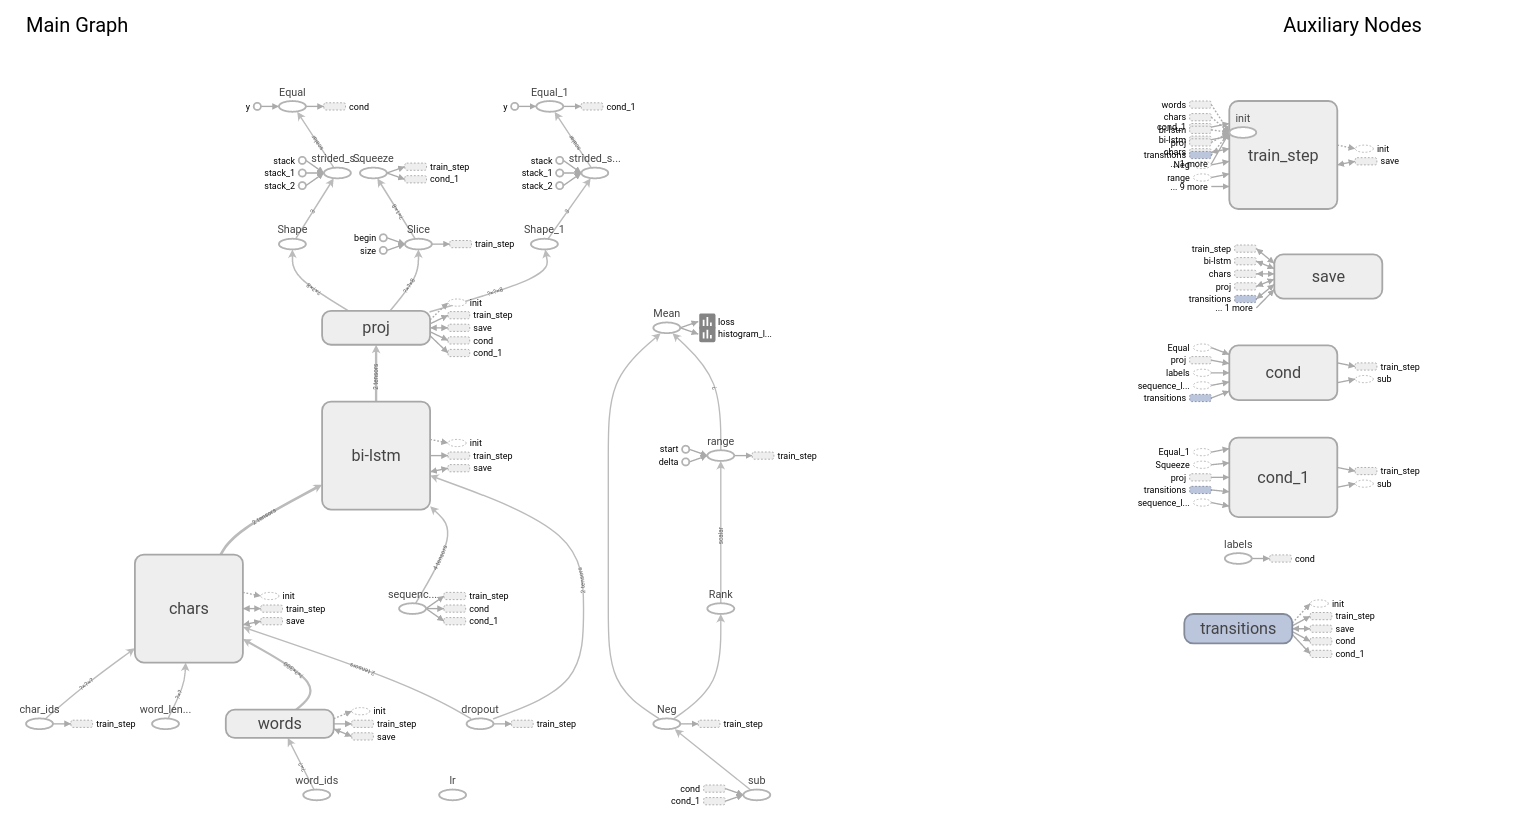
\includegraphics[width=6.5in]{images/finalGraph.png}
  \caption {Final graph}
  \label{fig:finalGraph}
\end{figure}

We now have the built-in network, now it has to be trained and tested.

\begin{lstlisting}[language=Python,caption={Train network}]
    def train(self, train: CoNLLDataset, dev: CoNLLDataset):
        best_score = 0
        n_epoch_no_improve = 0  # for early stopping
    
        for epoch in range(self.config.n_epochs):
            score = self._run_epoch(train, dev, epoch)
            self.config.lr *= self.config.lr_decay  # decay learning rate
    
            if score >= best_score:
                n_epoch_no_improve = 0
                best_score = score
                self.save_session()
            else:
                n_epoch_no_improve += 1
                if n_epoch_no_improve >= self.config.n_epoch_no_improve:
                    break
    
    def _run_epoch(self, train: CoNLLDataset, dev: CoNLLDataset, epoch) -> int:
        n_batches = (len(train) + self.config.batch_size - 1) // self.config.batch_size

        # iterate over dataset
        for i, (words, labels) in enumerate(minibatches(train, self.config.batch_size)):
            fd, _ = self.get_feed_dict(words, labels, self.config.lr, self.config.dropout)

            _, train_loss, summary = self.sess.run([self.train_op, self.loss, self.merged], feed_dict=fd)

        metrics = self._run_evaluate(dev)

        return metrics["f1"]
\end{lstlisting}

As mentioned above, the network will be fed with a small number of sentences of the same length. So for that we need a tool that uniformises sentences and characteristics too. In other words, to transforms the words in there ids based on the dictionary and bring them in the same form.

\begin{lstlisting}[language=Python,caption={Make embeddings}]
    def pad_sequences(sequences, sequences_length=None):
        sequences_length = max(
            map(lambda x: len(x) if type(x) is not int else 0, sequences)) if sequences_length is None else sequences_length
    
        seqs = []
        lengths = []
        for sequence in sequences:
    
            seq = fill_array(sequence if type(sequence) is not int else [sequence], sequences_length)
            length = len(sequence) if type(sequence) is not int else 0
    
            if type(sequence) is not int and type(sequence[0]) == list:
                max_length_word = max([max(map(lambda x: len(x), _seq)) for _seq in sequences])
    
                # seq = list(map(lambda x: [x] if type(x) == int else x, seq))
                seq, length = pad_sequences(seq, max_length_word)
    
            lengths += [length]
            seqs += [seq]
    
        return seqs, lengths
\end{lstlisting}

Now we can feed the network. For that need to fit placeholders dimensions.

\begin{itemize}
    \item word\_ids: (batch size, max length of sentence in batch)
    \item sequence\_lengths: (batch size)
    \item char\_ids: (batch size, max length of sentence in batch, max length of word in sentence)
    \item word\_lengths: (batch size, max length of sentence in batch)
    \item labels: (batch size, max length of sentence in batch)
\end{itemize}

\begin{lstlisting}[language=Python,caption={Feed network}]
    def get_feed_dict(self, words, labels=None, lr=None, dropout=None):

        char_ids, word_ids = zip(*words)

        word_ids, sequence_lengths = pad_sequences(word_ids)
        char_ids, word_lengths = pad_sequences(char_ids)

        # build feed dictionary
        feed = {
            self.word_ids: word_ids,
            self.sequence_lengths: sequence_lengths,
            self.char_ids: char_ids,
            self.word_lengths: word_lengths
        }

        if labels is not None:
            labels, _ = pad_sequences(labels)
            feed[self.labels] = labels

        if lr is not None:
            feed[self.lr] = lr

        if dropout is not None:
            feed[self.dropout] = dropout

        return feed, sequence_lengths
\end{lstlisting}

There are two types of evaluation for neural network, one based on exact match (f1) and index matching.

In statistical analysis of binary classification, the F1 score (also F-score or F-measure) is a measure of a test's accuracy. It considers both the precision p and the recall r of the test to compute the score: p is the number of correct positive results divided by the number of all positive results returned by the classifier, and r is the number of correct positive results divided by the number of all relevant samples (all samples that should have been identified as positive). The F1 score is the harmonic average of the precision and recall, where an F1 score reaches its best value at 1 (perfect precision and recall) and worst at 0.

\begin{equation*}
     F_1=2 * \frac {precision * recall} {precision + recall}
\end{equation*}

\begin{lstlisting}[language=Python,caption={Test network}]
    def _run_evaluate(self, test: CoNLLDataset):
        accs = []
        correct_preds, total_correct, total_preds = 0., 0., 0.
        for words, labels in minibatches(test, self.config.batch_size):
            labels_pred, sequence_lengths = self.predict_batch(words)

            for lab, lab_pred, length in zip(labels, labels_pred,
                                             sequence_lengths):
                lab      = lab[:length]
                lab_pred = lab_pred[:length]
                accs    += [a==b for (a, b) in zip(lab, lab_pred)]

                cond = lambda x: x[0] != self.config.vocab_tags[NONE]   

                lab_chunks = set(filter(cond, get_chunks(lab, self.config.vocab_tags)))
                lab_pred_chunks = set(filter(cond, get_chunks(lab_pred, self.config.vocab_tags)))

                correct_preds += len(lab_chunks & lab_pred_chunks)
                total_preds += len(lab_pred_chunks)
                total_correct += len(lab_chunks)

        p = correct_preds / total_preds if correct_preds > 0 else 0
        r = correct_preds / total_correct if correct_preds > 0 else 0
        f1 = 2 * p * r / (p + r) if correct_preds > 0 else 0
        acc = np.mean(accs)

        return {"acc": 100 * acc, "f1": 100 * f1}

    def predict_batch(self, words):

        fd, sequence_lengths = self.get_feed_dict(words, dropout=1.0)

        viterbi_sequences = []
        logits, trans_params = self.sess.run([self.logits, self.trans_params], feed_dict=fd)

        for logit, sequence_length in zip(logits, sequence_lengths):
            logit = logit[:sequence_length] 
            viterbi_seq, viterbi_score = tf.contrib.crf.viterbi_decode(logit, trans_params)
            viterbi_sequences += [viterbi_seq]

        return viterbi_sequences, sequence_lengths
\end{lstlisting}

\subsubsection{Tests}

Reteteau has been tested on several types of configurations. The best results were obtained with the following configurations.

\begin{lstlisting}[language=Python,caption={Network configurations}]
    n_epochs = 5
    dropout = 0.5  # rate to randomize
    batch_size = 20  # nb of sentence
    lr_method = "adam"
    lr = 0.001  # learn rate
    lr_decay = 0.9  # adjust learn rete
    n_epoch_no_improve = 3

    hidden_size_char_lstm = 100  # lstm on chars
    hidden_size_word_lstm = 300  # lstm on word embeddings
\end{lstlisting}

It is to be noted that the training of the network takes about 25 minutes with these configurations.

\begin{lstlisting}[language=Python,caption={Network results during training}]
    2018-04-15 00:31:01,504 - logger - INFO - Initializing tf session
    2018-04-15 00:31:02,658 - logger - INFO - Epoch 1 out of 5
    2018-04-15 00:36:10,565 - logger - INFO - acc 97.13 - f1 81.56
    2018-04-15 00:36:10,990 - logger - INFO - - new best score!
    2018-04-15 00:36:10,990 - logger - INFO - Epoch 2 out of 5
    2018-04-15 00:41:07,991 - logger - INFO - acc 97.67 - f1 86.18
    2018-04-15 00:41:08,586 - logger - INFO - - new best score!
    2018-04-15 00:41:08,586 - logger - INFO - Epoch 3 out of 5
    2018-04-15 00:46:02,616 - logger - INFO - acc 97.97 - f1 88.25
    2018-04-15 00:46:03,339 - logger - INFO - - new best score!
    2018-04-15 00:46:03,339 - logger - INFO - Epoch 4 out of 5
    2018-04-15 00:50:58,869 - logger - INFO - acc 98.18 - f1 89.35
    2018-04-15 00:50:59,477 - logger - INFO - - new best score!
    2018-04-15 00:50:59,477 - logger - INFO - Epoch 5 out of 5
    2018-04-15 00:55:53,944 - logger - INFO - acc 98.22 - f1 89.87
    2018-04-15 00:55:54,455 - logger - INFO - - new best score!
\end{lstlisting}

One of the results obtained after training is the following
\begin{equation*}
    acc = 97.21;
    f1 = 85.23;
\end{equation*}


\begin{figure}[H]
  \centering
  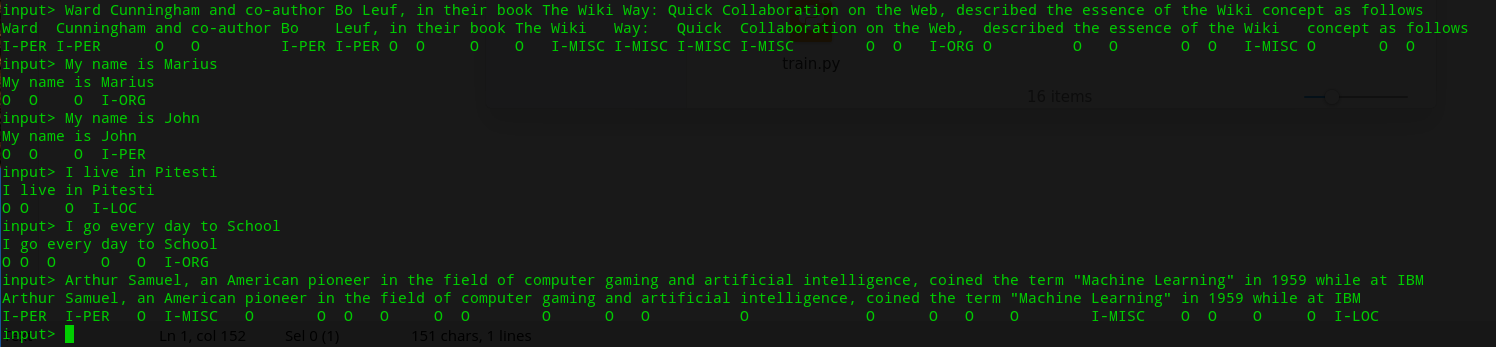
\includegraphics[width=6.5in]{images/interactive.png}
  \caption {Some of the interactive results}
\end{figure}

Here's how the loss diagram shows:

\begin{figure}[H]
  \centering
  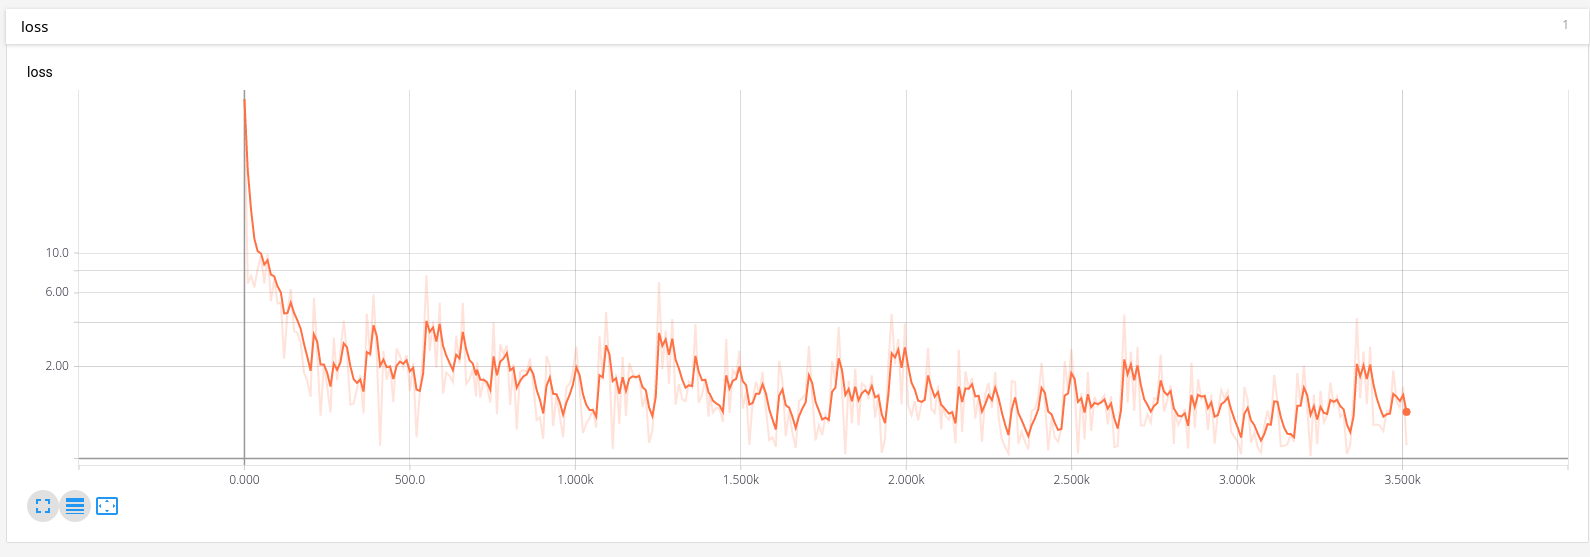
\includegraphics[width=6.5in]{images/loss.png}
  \caption {Loss diagram}
\end{figure}

Tensor board also provides a way of representing words. You can also see the links between Gloved words.

\begin{figure}[H]
  \centering
  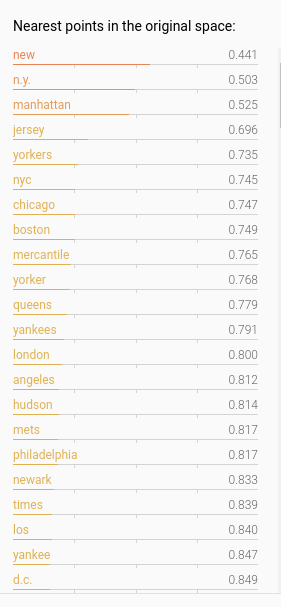
\includegraphics[width=2.5in]{images/york.png}
  \caption {Distance for word "York"}
\end{figure}

    
    \newpage
    \section*{Conclusion}
\addcontentsline{toc}{section}{Conclusion}

The work done represents a special incursion in the fundamental field of neural networks, both by presenting the main elements that define this field and by the illustrative character of the experimental experimentation of the neural algorithms performance in applications of great interest in the current researches.

In the paper were presented the notions defining the field of neural networks, by describing the neuron structure, highlighting the comparison between the artificial and the human neuron, the possible training possibilities for the unilateral or multilayer neuronal architectures by using information about the correct answers associated with the data training and so we have supervised learning, by determining as far as possible the final clusters that induce unsupervised learning, as well as enumerating the main areas of applicability. It is possible to specify the numerous applications present in the field of form recognition with the use of neural network-specific training algorithms.

The tensorflow framework was used in the elaboration of the paper. It provides standard deployments for a wide range of optimizations for neural networks, architecture, and more. We also used the uncontrolled neural network GloVe to train words and find correspondence between them. These tools have been applied to find and classify names in texts.



    \newpage
    \bibliographystyle{plain}
    \bibliography{references}
\end{document}
